\subsection{Выбор используемого протокола}

Для разработки необходимо выбрать способ удаленного доступа, который будет
использоваться в системе. Так как выбор зависит от серверной ОС, выбор оптимального
варианта связан с доступными на Windows протоколами.

Основной протокол, используемый в Windows — RDP (Remote Desktop Protocol). Клиент RDP
доступен во всех редакциях Windows, начиная с Windows XP, что позволяет использовать
любой компьютер кафедры в качестве тонкого клиента (см. рисунок \ref{pic:mstsc_xp}).
Однако, RDP-клиенты существуют для многих платформ, в том числе для Linux.

\begin{figure}[h]
    \center
    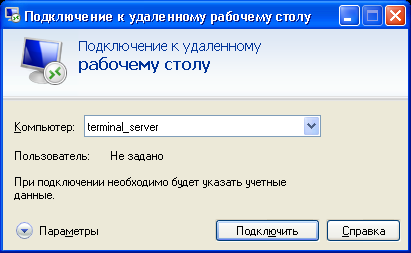
\includegraphics[height=8cm]{mstsc_xp}
    \caption{Окно RDP-клиента, встроенного в Windows XP}
    \label{pic:mstsc_xp}
\end{figure}

\subsection{Клиентское ПО}

В качестве клиентской ОС выбран стандартный для Raspberry Pi дистрибутив Linux Raspbian,
основанный на Debian \cite{ref:raspbian}.
Дистрибутив поддерживается Raspberry Pi Foundation и рекомендован к установке.
К его преимуществам можно отнести открытый исходный код, простоту установки и удобство 
настройки. 
Актуальной на момент разработки была версия Buster, вышедшая в феврале 2020 года.

Для RDP-клиента использовано ПО \textit{FreeRDP}, актуальной на момент разработки версии
2.0.0 \cite{ref:freerdp}. Данный программный продукт позволяет осуществлять подключение
к RDP-серверам любой версии, просто и гибко настраивается для получения оптимальной
производительности.  Так как исходный код открыт, есть возможность скомпилировать
бинарный файл для нужной архитектуры (в рассматриваемом проекте используется архитектура
ARM).
